
\documentclass[11pt, a4paper]{report}
\usepackage{graphicx}
\usepackage{fullpage}
\usepackage{url}
\usepackage{listings}
\pagestyle{headings}

\headsep = 25pt
\begin{document}

\title{\Huge IndividualTesting Report }
\author{Li Shikai\\ \\ID: a1214223}
\date{21 October 2012}
\maketitle
\pagebreak
\oddsidemargin -0.5 cm
\evensidemargin -0.5 cm
\textwidth 15 cm
\topmargin -1.2 cm
\textheight 25 cm
\tableofcontents

\chapter{Introduction of the Test Plan}
This test project will concentrate on Menu testing, meanly test the availability of Menu Items in different states, include default state, New Map Initial state, and Robot Connected state. Also there will be two test cases about text field and robot current coordinate displayed on GUI.
\section{Introduction of Menu Test}
\begin{enumerate}
\item The default is when the GUI is start to run and without any further interruption. Most of Menu item operation is not available to to select. I am plan to test, whether the Menu item has been set correctly.
\item The new map initial state is when addNew button has been clicked and new map has been initialed. Some Menu item will unlock from disable statue. i will test if these menu unlocked as we expected.
\item The Robot Connected state is When the robot is connected though Menu or connect button. Most of Menu will enable, but few Menu will disable when connected. Also, mode change test will include in this test case for testing availability status change of some Menu items.
\end{enumerate}
\section{Introduction of TextField Test}
System log is a text field located on the top right of GUI panel. It return system information from robot, XML file and user operation. This test will checking the correctness of text display, and Print Stream from system.
\section{Introduction of Robot Current Coordinate Test}
Robot coordination labels are located on the bottom left of GUI panel. It will performance robot coordination real time updating after connection is established. This test case will test accuracy of coordination when map initialed and position altered.
\begin{enumerate}
\item Forward Operation. Using GUI to control the forward movement(it means move to the north of the map) of the robot, mainly check whether or not the robot is able to move one pixel when user presses forward button every one time.
\item TurnLeft Operation. Using GUI to control the turnLeft movement of the robot. When user uses the GUI to let the robot turn left, I need to make sure the robot is able to turn left 90 degrees.
\end{enumerate}
\chapter{Test Plan and Specific Test Case}
\section{Test different GUI states}
\begin{enumerate}
\item The function of GUI is build a simple and easily understood interface, let user give instructions to system, and system will reaction in a proper way. So this test will concentrate on the different constraints are set to Menu of GUI in each state. And how user can interact with it.
\item System log is the primary way user can get information return from system, and confirm the correctness of current operation. So all the information should be catched completely. In this case, i will test three ways to update system log, include two functions and default System.out.print().
\item Although user can get robot position just by looking at map panel, robot coordination is still a good way to get precise robot current position. So this test case mainly test the accurate and real time update when map has been changed.

\end{enumerate}
\section{Testing Tool and Operating System}
\begin{itemize}
\item Eclipse SDK
\item Version: 4.2.0
\item Build id: I20120608-1400
\item JUnit
\item Operating System: Windows 7
\end{itemize}
\section{Test1: Default Menu State}
\subsection{Test method}
\begin{itemize}
\item Method: MenuBarInitail(). This method is called when a new Map is Initialed.
\end{itemize}
\subsection{Description:}
When the program is started. MenuBarInitail() will be called by initial() function to build menu part of GUI. This function will give the default constraint of each menu item, like user are not expected to save a map if then did not even initial a new map. So i will use java.awt.Component.isEnabled() to test whether the Menu items are disabled as we expect.
 \begin{center}
 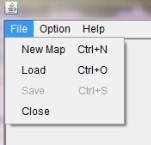
\includegraphics[width=11.20cm]{FileMenuDefault}
 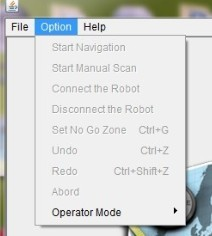
\includegraphics[width=11.20cm]{OptionMenuDefault}
\end{center}
\subsection{Pass criteria}
\begin{itemize}
\item As the picture shows, most items in File menu are available in default stage, except Save map option, which are not permit to select without precondition new map or load map.
\item For Option menu, except change operator mode, all the other items are not able to be select. Those items are all about instruction to robot explore, so we want user to use it after the connection has been established.  
\end{itemize}
\subsection{Test Type}
JUnit test
\subsection{Pass or Fail}
Pass

\section{Test2: New map initial State}
\subsection{Method:}
\begin{itemize}
\item class NewMapStart()
\end{itemize}
\subsection{Description:}
The second state is New map initial, i plan to use javax.swing.AbstractButton.doClick() method to simulate a mouse click to addNew button then do the same operation to Confirm button to accept default map arguments and then Initial a new map. Enter the second state, we do the same test as default state, but change some expecting result to test the Menu item constraints.
\begin{center}
 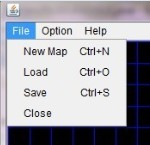
\includegraphics[width=10cm]{FileMenuNewMapInitial}
 \end{center}
 \begin{center}
 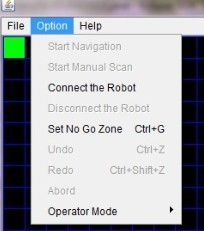
\includegraphics[width=10cm]{OptionMenuNewMapInitial}
\end{center}
\subsection{Pass criteria}
\begin{itemize}
\item As we can see all the items are enabled in File menu. So we use AssertTrue to test those items.
\item After a map has been initial, we expect user are able connect robot, also no go zone can be set before exploring. AssertTrue are used to measure those two items.
\end{itemize}
\subsection{Test Type}
JUnit Test
\subsection{Pass or Fail}
Pass
\section{Test3: Robot connection State}
\subsection{Test method}
\begin{itemize}
\item listener ConnectionListener().
\end{itemize}
\subsection{Description}
After initial a new map, we do the same operation to button bluetoothConnection for connecting the robot. Because we are not really establish the connection, nullPointerException is expected in this test. After test connection state menu items constraint, i will test the change when control mode switch.
 \begin{center}
  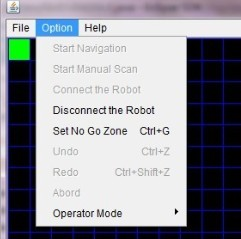
\includegraphics[width=11.20cm]{OptionMenuConnection}
  \end{center}
  \begin{center}
 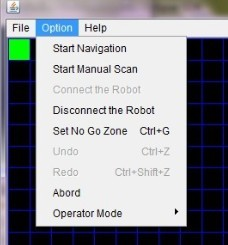
\includegraphics[width=11.20cm]{AutoModeMenu}
 \end{center}
 \begin{center}
 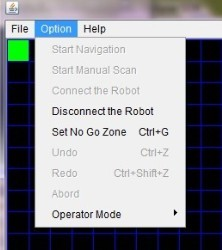
\includegraphics[width=11.20cm]{ManualModeMenu}
\end{center}
\subsection{Pass criteria}
\begin{itemize}
\item After robot connected, disconnect menu items will unlock. Meanwhile connect option will disable. Until next map initialed.
\item To automatic test mode change i implement a thread to run Java.awt.Robot.keyPressed() to accept JOptionPane mode switch option. 
\item In auto mode, we assertTrue() start navigation, start manual scan and abord. On the contrary we use assertFalse to meansure those three items in manual mode.

\end{itemize}
\subsection{Test Type}
JUnit Test
\subsection{Pass or Fail}
Pass
\section{Test4: TextField Test}
\subsection{Test method}
\begin{enumerate}
\item public void LEGOGUI.setText(String str). 
\item public void LEGOGUI.append(String str)
\end{enumerate}
\subsection{Description}
There are three ways to update text field. Two are through function call. One is print stream from System.out.print();
\begin{center}
  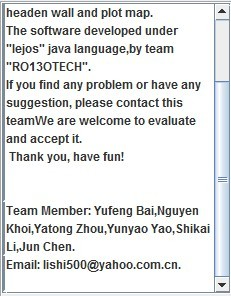
\includegraphics[width=11.20cm]{LogDisplay}
\end{center}
\subsection{Pass criteria}
\begin{enumerate}
\item First test append(String) function. This function will append the input String with a new line on the end of existing String. So we first get the current text from text field though textField.getText(), then call append function to append a string on text Field. After that we assertEquals() old text plus a new line plus text we append with current text field text. 
\item Similar operation, but setText(String) is set text field as the given String, so we just assertEquals() given text with getText();
\item We transfer the output of System.out.print() from terminal to text field, in TextAreaPrintStream class. It perform just as append(String) function, so the testing method is mostly same.
\end{enumerate}
\subsection{Test Type}
Junit test
\subsection{Pass or Fail}
Pass
\section{Robot Coordination Test}
\subsection{Description:}
When the Robot position changed, the coordinate of robot will change with it, So test if the current position of robot(map.getCurrentPixel().getxPos()/.getyPos()) is same with map panel display.
\begin{center}
  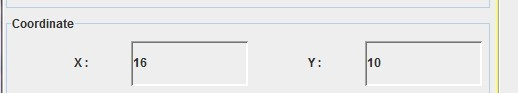
\includegraphics[width=11.20cm]{coordinate}
\end{center}
\subsection{Pass Criteria}
\begin{itemize}
\item First i will test if the coordination display correctly when the new map is initialed. With the default setting robot start position (0,0).
\item Then i will test if the map changed, the robot current position has been altered, whether the coordination panel change with it.
\end{itemize}
\subsection{Testing Type}
Junit test
\subsection{Pass or Fail}
Pass

\newpage
\appendix
\chapter{the GUI test}
\begin{lstlisting}
package Tests;

import static org.junit.Assert.*;
import java.awt.event.KeyEvent;

import GUI.*;
import org.junit.Test;



public class MenuTestCase {

	@Test
	public void testDefaultMenuEnabled(){
		
		LEGOGUI lego = new LEGOGUI();
		
		//test FIleMenu load ,save statues
		assertTrue(lego.file_new.isEnabled());
		assertTrue(lego.file_open.isEnabled());
		assertFalse(lego.file_save.isEnabled());
		assertTrue(lego.file_close.isEnabled());
		
		//test OptionMenu initial statues
		assertFalse(lego.start_navigation.isEnabled());
		assertFalse(lego.manual_scan.isEnabled());
		
		assertFalse(lego.connect_connectRob.isEnabled());
		assertFalse(lego.connect_disconRob.isEnabled());
		
		assertFalse(lego.file_setNoGoZone.isEnabled());
		assertFalse(lego.file_UndoNoGoZone.isEnabled());
		assertFalse(lego.file_RedoNoGoZone.isEnabled());
		assertFalse(lego.abordMisson.isEnabled());
			
	}
	@Test
	public void testNewMapInitialedMenuEnabled(){
		LEGOGUI lego = new LEGOGUI();
		// set addNew map clicked;
		// set new map panel confirm button clicked
		lego.addNew.doClick ();
		lego.nms.mi.Confirm.doClick();
		
		//test FIleMenu load ,save statues
		assertTrue(lego.file_save.isEnabled());// file is enabled
				
		//test OptionMenu initial statues
		assertFalse(lego.start_navigation.isEnabled());
		assertFalse(lego.manual_scan.isEnabled());
				
		assertTrue(lego.connect_connectRob.isEnabled()); // connect_robot is enabled
		assertFalse(lego.connect_disconRob.isEnabled());
				
		assertTrue(lego.file_setNoGoZone.isEnabled());  //set no go zone is enabled
		assertFalse(lego.file_UndoNoGoZone.isEnabled());
		assertFalse(lego.file_RedoNoGoZone.isEnabled());
		assertFalse(lego.abordMisson.isEnabled());
		
	}
	
	@Test//(expected = NullPointerException.class , timeout=1000)
	public void testConnectedMenuEnabled() {
		final LEGOGUI lego = new LEGOGUI();
		// set addNew map clicked;
		// set new map panel confirm button clicked
		lego.addNew.doClick ();
		lego.nms.mi.Confirm.doClick();		
		lego.bluetoothConnection.doClick();
		
		//test FIleMenu load ,save statues
		assertTrue(lego.file_save.isEnabled());// file is enabled
				
		//test OptionMenu initial statues
		assertFalse(lego.start_navigation.isEnabled());
		assertFalse(lego.manual_scan.isEnabled());
				
		assertFalse(lego.connect_connectRob.isEnabled()); // connect_robot is enabled
		assertTrue(lego.connect_disconRob.isEnabled());
				
		assertTrue(lego.file_setNoGoZone.isEnabled());  //set no go zone is enabled
		assertFalse(lego.file_UndoNoGoZone.isEnabled());
		assertFalse(lego.file_RedoNoGoZone.isEnabled());
		assertFalse(lego.abordMisson.isEnabled());
		
		
		// thread automatic click enter, to ensure select right mode
		new Thread(){
        	public void run(){
        		int i = 0;
        		while(i< 10){
					lego.robot.keyPress(KeyEvent.VK_ENTER);
					try {
						Thread.sleep(100);
					} catch (InterruptedException e) {
						e.printStackTrace();
					}
					i++;
				}
        	}    	
        }.start();
     // click auto button
		lego.auto.doClick();
				
		assertTrue(lego.start_navigation.isEnabled());
		assertTrue(lego.manual_scan.isEnabled());
		assertTrue(lego.abordMisson.isEnabled());
		// click manual button
		lego.manual.doClick();
		assertFalse(lego.start_navigation.isEnabled());
		assertFalse(lego.manual_scan.isEnabled());
		assertFalse(lego.abordMisson.isEnabled());
	}
	@Test
	public void testTestField() {
		LEGOGUI lego = new LEGOGUI();
		
		// test append function for JTextFiled
		String text = lego.text.getText();
		String append = "append";
		lego.append(append);
		assertEquals(text+"\n"+append,lego.text.getText());
					
		// test setText function for JTextFiled
		String setText = "setText";
		lego.setText(setText);
		assertEquals(setText,lego.text.getText());
		
		// test TextAreaPrintStream
		String Stream = "Stream";
		text = lego.text.getText();
		System.out.println(Stream);
		assertEquals(text+Stream,lego.text.getText().trim());
	}
	
	@Test
	public void testRobotCurrentCoordinateValue() {
		LEGOGUI lego = new LEGOGUI();
		lego.addNew.doClick ();
		lego.nms.mi.Confirm.doClick();
		
		// first test default robot coordinate x and y value
		// and the label relate display on GUI
		int posX, posY;
		posX = lego.map.getCurrentPixel().getxPos();
		posY = lego.map.getCurrentPixel().getyPos();
		assertEquals(0,posX);
		assertEquals(0,posX);
		assertEquals(0,Integer.parseInt(lego.xValue.getText().trim()));
		assertEquals(0,Integer.parseInt(lego.yValue.getText().trim()));
		
		// then test when robot current position has been changed
		// and the label relate display on GUI
		lego.map.setCurrentPixel(lego.map.findPixel(5,8));
		posX = lego.map.getCurrentPixel().getxPos();
		posY = lego.map.getCurrentPixel().getyPos();
		assertEquals(5,posX);
		assertEquals(8,posY);
		lego.updateCoordinateValue();
		assertEquals(5,Integer.parseInt(lego.xValue.getText().trim()));
		assertEquals(8,Integer.parseInt(lego.yValue.getText().trim()));
	}			
}
\end{lstlisting}
\chapter{Glossary and Reference}
\section{Glossary}
\begin{itemize}
\item GUI: Graphical User Interface.
\item Junit: is a unit testing framework for the Java programming language.
\end{itemize}
\section{Reference}
\begin{lstlisting}
http://en.wikipedia.org/wiki/JUnit
http://docs.oracle.com/javase/1.4.2/docs/api
\end{lstlisting}
\end{document}
